
This appendix consists of additional details regarding Chapters 3 and 4.

\section{Optimal representation of $\widetilde{\mathbf{W}}$}
\newtheorem{name2}{Theorem 2.}
\begin{name2}
\label{approx}
The optimal binary weight $\widetilde{\mathbf{W}}$ which minimizes the error function $\mathbf{J}$ is
$$\widetilde{\mathbf{W}} = \alpha \mathbf{e} + \beta \mathbf{(1-e)} \\$$
where $\; \alpha =\frac{\mathbf{W}^{T}\mathbf{e}}{K} \;$, $\; \beta = \frac{\mathbf{W}^{T}\mathbf{(1-e)}}{n-K} \;$ and the optimal $\mathbf{e}^\ast$ is $\;  \mathbf{e}^\ast  = \underset{\mathbf{e},K}{\mathrm{argmax}} (\frac{ \parallel \mathbf{W}^T\mathbf{e} \parallel^{2}}{K} + \frac{\parallel \mathbf{W}^{T}\mathbf{(1-e)}\parallel^{2}}{n-K})$
\end{name2}

{\bf Proof:} The approximated weight vector $\widetilde{\mathbf{W}}=[\alpha \alpha \ldots \beta  \alpha  \ldots \beta \beta$] can be decomposed as:
$$[\alpha \alpha \ldots \beta  \alpha  \ldots \beta \beta] = \alpha \cdot [ 1 1 \ldots 0  1  \ldots 0 0 ] + \beta \cdot [ 0 0 \ldots 1  0  \ldots 1 1 ]$$ 
where without loss of generality, $\mathbf{e} \in \{0,1\}^n, \mathbf{e}^T\mathbf{e} >  0, \mathbf{e} \in \{0,1\}^n, (\mathbf{1-e})^T(\mathbf{1-e}) >  0$ and $\alpha,\beta \in \mathbb{R}$. This is because the trivial case where $\mathbf{e} = \mathbf{0}$ or $\mathbf{e} = \mathbf{1}$ is covered by substituting  $\alpha = \beta$ instead and the equation is independent of $\mathbf{e}$.
We have to find the values of $\alpha$ and $\beta$ which would be the best approximation of this vector. \\
Let us define the error function $\mathbf{J} = \mathbf{W} - (\alpha \cdot \mathbf{e} + \beta \cdot (\mathbf{1-e}))$.
We have to minimize $\parallel \mathbf{J} \parallel^2 = \mathbf{E}$, where:
\begin{dmath}
\mathbf{E} = (\mathbf{W} - (\alpha \cdot \mathbf{e} + \beta \cdot (\mathbf{1-e})))^T(\mathbf{W} - (\alpha \cdot \mathbf{e} + \beta \cdot (\mathbf{1-e}))) \end{dmath}
\begin{dmath}
\mathbf{E} = \mathbf{W}^{T}\mathbf{W} + \alpha^2 \cdot \mathbf{e}^T\mathbf{e} + \beta^2\mathbf{(1-e)}^T \mathbf{(1-e)} \\ - 2\alpha \cdot \mathbf{W}^T\mathbf{e} - 2\beta \cdot \mathbf{W}^T(\mathbf{1-e}) + 2\alpha \beta \mathbf{e}^{T}\mathbf{(1-e)}
\end{dmath}
where $\mathbf{e}^T\mathbf{e} = K$, then $(\mathbf{1-e})^T(\mathbf{1-e}) = n-K$ and $\mathbf{e}^{T}\mathbf{(1-e)} = 0$. Substituting these in, we get
\begin{equation}\mathbf{E} =  \mathbf{W}^{T}\mathbf{W} + \alpha^2 K + \beta^2 (n-K) -\\ 2\alpha \cdot \mathbf{W}^T\mathbf{e} - 2\beta \cdot \mathbf{W}^T(\mathbf{1-e}) \label{wformulation} 
\end{equation}
We minimize this equation with respect to $\alpha$ and $\beta$ giving us:

\begin{equation}\frac{\partial \mathbf{E}}{\partial \alpha} = 0 , \frac{\partial \mathbf{E}}{\partial \beta} = 0 \end{equation}
Solving the above, we get the equations:
$$ \frac{\partial \mathbf{E}}{\partial \alpha} = 2 \alpha K - 2 \cdot \mathbf{W}^T\mathbf{e} = 0 $$ $$ \frac{\partial \mathbf{E}}{\partial \beta} = 2 \beta (n-K) - 2 \cdot \mathbf{W}^T(\mathbf{1-e}) = 0  $$
We can get the values of $\alpha$ and $\beta$ from the above equations.
$$ \alpha = \frac{\mathbf{W}^T\mathbf{e}}{K} , \beta = \frac{\mathbf{W}^T(\mathbf{1-e})}{(n-K)} $$ 
Then substituting the values of $\alpha$ and $\beta$ in equation \ref{wformulation}, we get
\begin{dmath} 
\mathbf{E} = \parallel \mathbf{W} ||^2 + \frac{ \parallel \mathbf{W}^T\mathbf{e} \parallel^{2}}{K} + \frac{\parallel \mathbf{W}^{T}\mathbf{(1-e)}\parallel^{2}}{n-K} - 2\frac{\parallel \mathbf{W}^{T}\mathbf{e} \parallel^{2}}{K} - 2\frac{\parallel \mathbf{W}^{T}\mathbf{(1-e)}\parallel^{2}}{n-K} 
\end{dmath}
\begin{dmath}
\mathbf{E} = \parallel \mathbf{W} ||^2 - (\frac{ \parallel \mathbf{W}^T\mathbf{e} \parallel^{2}}{K} + \frac{\parallel \mathbf{W}^{T}\mathbf{(1-e)}\parallel^{2}}{n-K})
\end{dmath}
In the above equation, we want to minimize $\mathbf{E}$. Since $\mathbf{W}$ is a given value, we need maximize the second term to minimize the expression. For a given $K$, $\mathbf{e_K} = sgn(\mathbf{T_k})$ where $\mathbf{T_k} = topk(\mathbf{W},K)$.
Here, $topk(\mathbf{W},K)$ represents the top $K$ values of $\mathbf{W}$ corresponding to either the largest positive $K$ values or the largest negative $K$ values, which remain as is whereas the rest are converted to zeros.

$$ \mathbf{e}^\star  = \underset{\mathbf{e,K}}{\mathrm{argmax}} (\frac{ \parallel \mathbf{W}^T\mathbf{e} \parallel^{2}}{K} + \frac{\parallel \mathbf{W}^{T}\mathbf{(1-e)}\parallel^{2}}{n-K}) $$

\noindent  Selecting the $topk(\mathbf{W},K)$ would be optimal since $||\mathbf{W}^{T}\mathbf{e}||$ and $||\mathbf{W}^{T}\mathbf{(1-e)}||$ are both maximized on selecting either the largest $K$ positive values or the largest $K$ negative values. Hence, this allows us to select the optimal $\mathbf{e}$ given a $K$.
With this, we obtain the optimal $\mathbf{e}$.

\section{Gradient derivation}

$$W \approx \widetilde{\mathbf{W}} = \alpha \mathbf{e} + \beta \mathbf{(1-e)} \\$$
$$where\; \alpha =\frac{\mathbf{W}^{T}\mathbf{e}}{K} \; and \; \beta = \frac{\mathbf{W}^{T}\mathbf{(1-e)}}{n-K} \\$$
Let $\mathbf{T_k} = topk(\mathbf{W}, K)$, and $\widetilde{\mathbf{W}_{1}} = \alpha \mathbf{e}$, and $\widetilde{\mathbf{W}_{2}} = \beta \mathbf{(1-e)}$. \\
Considering $\alpha$, on substituting $e = sgn(T_k)$. \\
$$\alpha = \frac{\mathbf{W}^{T}\mathbf{e}}{K} \\$$
$$\therefore \alpha = \frac{\mathbf{W}^{T}sgn(\mathbf{T_k})}{K}$$
Hence, we have $\alpha = \frac{\mathbf{W}^{T}sgn(\mathbf{T_k})}{K}$ and similarly $\beta = \frac{\mathbf{W}^{T}(1-sgn(\mathbf{T_k}))}{n-K}$. Putting these back in $\widetilde{\mathbf{W}}$, we have, \\
\begin{dmath}
\therefore \widetilde{\mathbf{W}} = \frac{\mathbf{W}^{T}sgn(\mathbf{T_k})}{K}\circ sgn\mathbf{(T_k)} + \frac{\mathbf{W}^{T}(1-sgn(\mathbf{T_k}))}{n-K}\circ (1-sgn\mathbf{(T_k)})
\end{dmath}
Now, we compute the derivatives of $\alpha$ and $\beta$ with respect to $\mathbf{W}$,
$$\frac{d\alpha }{d\mathbf{W}} = \frac{d(\mathbf{W}^{T}sgn(\mathbf{T_k}))}{d\mathbf{W}}.\frac{1}{K} \\$$
$$\frac{d\alpha }{d\mathbf{W}} = \frac{d(\mathbf{T_k}^{T}sgn(\mathbf{T_k}))}{d\mathbf{W}}.\frac{1}{K} \\$$
\begin{dmath}
\frac{d\alpha }{d\mathbf{W}} = \frac{d(||\mathbf{T_k}||_{l1})}{d\mathbf{W}}.\frac{1}{K}=\frac{sgn(\mathbf{T_k})}{K}
\end{dmath}
Similarly, \\
\begin{dmath}
\frac{d\beta}{d\mathbf{W}} = \frac{d(||\mathbf{W}-\mathbf{T_k}||_{l1})}{d\mathbf{W}}.\frac{1}{n-K}=\frac{sgn(\mathbf{W}-\mathbf{T_k})}{n-K}
\end{dmath}
Now, $\widetilde{\mathbf{W}_{1}} = \alpha \mathbf{e}$ therefore,
$$\frac{d\widetilde{\mathbf{W}_{1}}}{d\mathbf{W}} = e \frac{d\alpha}{d\mathbf{W}} + \alpha \frac{d\mathbf{e}}{d\mathbf{W}} $$
$$\therefore \frac{d\widetilde{\mathbf{W}_{1}}}{d\mathbf{W}} = \frac{sgn(\mathbf{T_k})}{K}\circ sgn(\mathbf{T_k}) + \alpha.STE(\mathbf{T_k})$$
With this, we end up at the final equation for $\widetilde{\mathbf{G_1}} = \frac{d\widetilde{\mathbf{W}_{1}}}{d\mathbf{W}}$ as mentioned in the paper,
\begin{dmath}
\therefore \widetilde{\mathbf{G_1}} = \frac{sgn(\mathbf{T_k})}{K} \circ sgn(\mathbf{T_k}) + \frac{||\mathbf{T_k}||_{l1}}{K}STE(\mathbf{T_k})
\end{dmath}
Considering the second term $\widetilde{\mathbf{W}_2}$, we have,
$$\frac{d\widetilde{\mathbf{W}_{2}}}{d\mathbf{W}} = \mathbf{(1-e)} \frac{d\beta}{d\mathbf{W}} + \beta \frac{d\mathbf{(1-e)}}{d\mathbf{W}}$$
$$\therefore \frac{d\widetilde{\mathbf{W}_{2}}}{d\mathbf{W}} = \frac{sgn(\mathbf{W}-\mathbf{T_k})}{n-K} \circ (1-sgn(\mathbf{T_k})) + \beta.STE(\mathbf{W}-\mathbf{T_k})$$
This provides us $\widetilde{\mathbf{G_2}} = \frac{d\widetilde{\mathbf{W}_{2}}}{d\mathbf{W}}$ as mentioned in the paper,
\begin{dmath}
\widetilde{\mathbf{G_2}} = \frac{sgn(\mathbf{W}-\mathbf{T_k})}{n-K} \circ (1-sgn(\mathbf{T_k})) + \frac{||\mathbf{W}-\mathbf{T_k}||_{l1}}{n-K}.STE(\mathbf{W}-\mathbf{T_k})
\end{dmath}
Together, we arrive at our final gradient $\widetilde{\mathbf{G}} = \frac{d\widetilde{\mathbf{W}}}{d\mathbf{W}}$,
\begin{dmath}
\widetilde{\mathbf{G}} = \widetilde{\mathbf{G_1}} + \widetilde{\mathbf{G_2}}
\end{dmath}

\section{Binary Networks as Approximators}
\noindent We define $m_{k}$ as the number of neurons required to approximate a polynomial of $n$ terms, given the network has a depth of $k$. We show that this number is bounded in terms of $n$ and $k$.
\begin{theorem}
For $p(x)$ equal to the product $x_1x_2\cdots x_n$, and for any $s$ with all nonzero Taylor coefficients, we have:
\begin{equation}
m_k(p, s) = \mathcal{O}\left(n^{(k-1)/k}\cdot 2^{n^{1/k}}\right).\label{eqn:constantlayers}
\end{equation}
\label{thm:constantlayers}
\end{theorem}
{\bf Proof:} We construct a binary network in which groups of the $n$ inputs are recursively multiplied.  The $n$ inputs are first divided into groups of size $b_1$, and each group is multiplied in the first hidden layer using $2^{b_1}$ binary neurons (as described in \cite{lin2017does}).  Thus, the first hidden layer includes a total of $2^{b_1}n/b_1$ binary neurons. This gives us $n/b_1$ values to multiply, which are in turn divided into groups of size $b_2$.  Each group is multiplied in the second hidden layer using $2^{b_2}$ neurons.  Thus, the second hidden layer includes a total of $2^{b_2}n/(b_1b_2)$ binary neurons.

We continue in this fashion for $b_1, b_2, \ldots, b_k$ such that $b_1b_2\cdots b_k = n$, giving us one neuron which is the product of all of our inputs.  By considering the total number of binary neurons used, we conclude
\begin{equation}
m_k(p, s) \le \sum_{i = 1}^k \frac{n}{\prod_{j = 1}^i b_j} 2^{b_i} = \sum_{i = 1}^k \left(\prod_{j = {i + 1}}^k b_j\right) 2^{b_i}.
\label{eqn:branching}
\end{equation}
Setting $b_i = n^{1/k}$, for each $i$, gives us the desired bound (\ref{eqn:constantlayers}).

\section{Expressibility of Binary Networks}
\noindent A binary neural network (a network with weights having only two possible values, such as $+1$ and $-1$) with a single hidden layer of $m$ binary-valued neurons that approximates a product gate for $n$ inputs can be formally written as a choice of constants $a_{ij}$ and $w_j$ satisfying
\begin{equation}
\sum_{j=1}^m w_j \sigma\left(\sum_{i=1}^n a_{ij} x_i\right) \approx \prod_{i=1}^n x_i. \label{goal}
\end{equation}

\noindent \cite{lin2017does} shows that $2^n$ neurons are sufficient to approximate a product gate with $n$ inputs - each of these weights are assigned, in the proof, a value of $+1$ or $-1$ before normalization, and all coefficients $a_{ij}$ also have $+1$/$-1$ values. This essentially makes it a binary network. Weight normalization introduces a scaling constant of sorts, $\frac{1}{2^{n}n!\sigma_{n}}$, which would translate to $\alpha$ in our representation, with its negative denoting $\beta$. \\
The above shows how binary networks are expressive enough to approximate real-valued networks, without the need for higher bit quantization.\\

\noindent Note: The above proofs for expressibility power have been borrowed from \cite{lin2017does}. 
\section{Experimental details}
\noindent We used the Adam optimizer for all the models with a maximum learning rate of 0.002 and a minimum learning rate of 0.00005 with a decay factor of 2. All networks are trained from scratch. Weights of all layers except the first were binarized throughout our experiments. Our FBin layer is structured the same as the XNOR-Net. We performed our experiments using a cluster of GeForce GTX 1080 Tis using PyTorch v0.2. 

\section{Experimental details}
Here we present additional experimental details for experiments in Chapter 3 and 4.
\subsection{Data processing} 
\noindent For all the datasets, we resized the images to $256\times 256$. A $224\times 224$ ($225\times 225$  for Sketchanet) sized crop was randomly taken from an image with standard augmentations such as rotation and horizontal flipping for TU-Berlin and Sketchy. In the TU-Berlin dataset, we use three-fold cross-validation which gives us a 2:1 train-test split to make our results comparable to all previous methods. For Sketchy, we use the training images for retrieval as the training images for classification and validation images for retrieval as the validation images for classification. We train models using the standard training and validation data for ImageNet-12. We report ten-crop accuracies for TU-Berlin and Sketchy, and only single-crop accuracies for ImageNet.

\subsection{Hyper-parameters} 
\noindent We use the PyTorch framework to train our networks. We used TU-Berlin and Sketchy datasets to evaluate Sketch-A-Net, ResNet-18, and SqueezeNet (v1.0) architectures, and ImageNet data on AlexNet and ResNet-18 architectures. Each FullBinConv block was structured as in XNOR-Net (Batchnorm-Activ-Conv-ReLU). Each WeightBinConv and Conv block has the standard convolutional block structure (Conv-Batchnorm-ReLU). Weights of all layers excepting the first were binarized throughout our experiments, unless specified otherwise. We used a dropout of 0.2 before the last two convolutional layers in Sketch-A-Net and AlexNet, and a dropout of 0.2 before the last layer in SqueezeNet except after an FBin layer as followed in the XNOR-Net paper. All networks were trained from scratch. We used the Adam optimizer for all the models with a maximum learning rate of 0.002 and a minimum of 0.00005 with a decay factor of 2.  We do not use a bias term or weight decay for FullBinConv and WeightBinConv layers. We used a batch size of 256 for all Sketch-A-Net models and a batch size of 128 for ResNet-18 and SqueezeNet models, the maximum size which fits in a 1080Ti GPU.\\

\section{FLOPs, Exploiting Filter Repetition and Computational Cost Calculation}
\noindent Layers of AlexNet and ResNet-18 models are shown in following Tables, along with the number of parameters and the corresponding FLOPs. The number of parameters of each layer for FPrec and Binary versions of the model shown in multiples of 0.1 million for the sake of clarity. The number of parameters in the Binary version of a given layer (\#BinParams) is calculated as follows: \\

\noindent FLOPs through each layer are given for FPrec, WBin, FBin and Hybrid versions, in multiples of 10 million. Except for the first layers, where weights are not binarized, the other layers have 58 times lesser FBin FLOP values due to enabling of XNOR/popcount operations. The number of repeated parameter values are also indicated and equivalent number of parameters in corresponding binarized layers are calculated as 
$$ \textnormal{\#WeightBinConvFLOPs} = \textnormal{\#FLOPs} \times (1-\textnormal{Repeated})$$
Then, we calculate the FLOPs in the FBin model by
$$\textnormal{\#FullBinConvFLOPs} = \frac{\textnormal{\#WbinFLOPs}}{58}$$
Further on, we select the parameters and FLOPs for each layer of the Hybrid models by selecting whether the layer is WeightBinConv or FullBinConv and pick the corresponding FLOPs.\\
The total number of parameters and FLOPs are calculated as the sum of individual layer FLOPs.

\section{Models used}
\noindent {\bf AlexNet:} A deep CNN that paved the way for most state-of-the-art CNN based models that exist today, and serves as a benchmark for comparison of network compression techniques.\\
{\bf ResNet-18:} A residual, implicitly compact model which is substantially deeper than previous standard models, that can be trained easily. \\
{\bf Sketch-A-Net:} A benchmark AlexNet-based model that was specifically engineered for sketches that beats human accuracy at sketch recognition, beating standard models fine-tuned on ImageNet which were unsuitable for sketch data. \\
{\bf SqueezeNet:} An explicitly compact CNN architecture achieving AlexNet accuracy with 50x fewer parameters.\\

\section{Model Architectures}
\noindent Figure \ref{fig:sketchanet} is a comparison of architectures of FPrec, WBin, FBin, and two Hybrid versions of the Sketch-A-Net model. The hybrids replace almost all convolutional layers with FullBinConv layers, except the ones towards the end, which are replaced with WeightBinConv layers. Figures \ref{fig:resnet} and \ref{fig:squeezenet} show a similar architectural comparison for ResNet-18 and SqueezeNet models.  

\section{Binarization-errors across layers }
In Figure 2 in the main paper, we use the proposed metric to measure binarization-error across layers in Sketch-A-Net, ResNet-18, and SqueezeNet models. We use stars to indicate where our algorithm replaces a layer with a WeightBinConv layer, and squares when our algorithm replaces a layer with a FullBinConv layer. Our metric is a function of approximation-error and the inverse of the number of FLOPs through the layer. Observe that our algorithm replaces layers with high error scores with FullBinConv layers, which occur towards the end, and weight-binarizes the rest. \\
The partitioning algorithm clustered these layers to mark them for full-binarization and weight-binarization. For example, in ResNet-18, the algorithm gave two major partitions - layers 2 to 11 in the first, and 12 to 16 in the next, with a significant difference in the cluster means. Hence, layers 12 to 16 were binarized for the hybrid model.




\begin{table}[t]
\centering
\resizebox{0.7\columnwidth}{!}{
\begin{tabular}{|l|c|c|c|c|c|c|c|c|}
\hline
{\bf Layers} &  \multicolumn{2}{c|}{\sc { \bf Parameters in 0.1M}} & \multicolumn{5}{c|}{\sc { \bf FLOPs }}\\
\hline
 & {\bf FPrec} & {\bf Bin} & {\bf FPrec} & {\bf Repeats} & {\bf WBin} & {\bf FBin} & {\bf Hybrid}\\
\hline
\multicolumn{8}{|c|}{\sc { \bf AlexNet}} \\
\hline
Conv1 & 0.23 & 0.232 & 10.54 & 0.00 & 10.54 & 10.54 & 10.54\\
Conv2 & 3.07 & 0.096 & 44.79 & 0 & 44.79 & 0.77 & 0.77\\
Conv3 & 6.64 & 0.207 & 14.95 & 0.71 & 4.34 & 0.07 & 0.07\\
Conv4 & 8.85 & 0.276 & 22.43 & 0.71 & 6.50 & 0.11 & 0.11\\
Conv5 & 5.90 & 0.184 & 14.95 & 0.60 & 5.98 & 0.10 & 0.10\\
Conv-FC1 & 377.49 & 11.796 & 3.77 & 0.00 & 3.77 & 0.07 & 3.77\\
Conv-FC2 & 167.77 & 5.243 & 1.68 & 0.00 & 1.68 & 0.03 & 1.68\\
Conv-FC3 & 40.96 & 1.280 & 0.41 & 0.00 & 0.41 & 0.41 & 0.41\\
Total & 610.90 & 19.316 & 113.53 &  & 78.01 & 12.11 & 17.47\\
\hline
\end{tabular}}
\caption{Layers of the AlexNet model, with the number of parameters and FLOPs for versions (WBin, Fbin, Hybrid, FPrec) of each. Also, the amount of unique parameters (a high number indicating high compressibility) is shown for each layer.}
\end{table}
\begin{table}[t]
\centering
\begin{tabular}{|l|c|c|c|c|c|c|c|c|}
\hline
{\bf Layers} &  \multicolumn{2}{c|}{\sc { \bf Parameters in 0.1M}} & \multicolumn{5}{c|}{\sc { \bf FLOPs }}\\
\hline
 & {\bf FPrec} & {\bf Bin} & {\bf FPrec} & {\bf Repeats} & {\bf WBin} & {\bf FBin} & {\bf Hybrid}\\
\hline
\multicolumn{8}{|c|}{\sc { \bf Sketch-A-Net}} \\
\hline
Conv1 & 0.23 & 0.232 & 7.26 & 0.00 & 7.26 & 7.26 & 7.26\\
Conv2 & 3.07 & 0.096 & 19.68 & 0.00 & 19.68 & 0.34 & 0.34\\
Conv3 & 6.64 & 0.207 & 6.64 & 0.58 & 2.80 & 0.05 & 0.05\\
Conv4 & 8.85 & 0.276 & 13.27 & 0.62 & 5.02 & 0.09 & 0.09\\
Conv5 & 5.90 & 0.184 & 13.27 & 0.61 & 5.19 & 0.09 & 0.09\\
Conv-FC1 & 47.19 & 1.475 & 0.64 & 0.00 & 0.64 & 0.01 & 0.64\\
Conv-FC2 & 2.62 & 0.082 & 0.03 & 0.00 & 0.03 & 0.00 & 0.03\\
Conv-FC3 & 1.28 & 0.040 & 0.05 & 0.00 & 0.05 & 0.05 & 0.05\\
Total & 75.77 & 2.593 & 60.84 &  & 40.68 & 7.89 & 8.54 \\
\hline
\end{tabular}
\caption{Layer descriptions of the Sketch-A-Net model.}
\end{table}
\begin{table}[t]
\centering
\begin{tabular}{|l|c|c|c|c|c|c|c|c|}
\hline
{\bf Layers} &  \multicolumn{2}{c|}{\sc { \bf Parameters in 0.1M}} & \multicolumn{5}{c|}{\sc { \bf FLOPs }}\\
\hline
 & {\bf FPrec} & {\bf Bin} & {\bf FPrec} & {\bf Repeats} & {\bf WBin} & {\bf FBin} & {\bf Hybrid} \\
\hline
\multicolumn{8}{|c|}{\sc { \bf ResNet-18}} \\
\hline
Conv1 & 0.09 & 0.094 & 11.80 & 0.00 & 11.80 & 11.80 & 11.80\\
Conv2 & 0.37 & 0.012 & 11.56 & 0.23 & 8.86 & 0.15 & 0.15\\
Conv3 & 0.37 & 0.012 & 11.56 & 0.31 & 7.99 & 0.14 & 0.14\\
Conv4 & 0.37 & 0.012 & 11.56 & 0.23 & 8.90 & 0.15 & 0.15\\
Conv5 & 0.37 & 0.012 & 11.56 & 0.23 & 8.86 & 0.15 & 0.15\\
Conv6 & 0.74 & 0.023 & 5.78 & 0.49 & 2.92 & 0.05 & 0.05\\
Conv7 & 1.47 & 0.046 & 11.56 & 0.39 & 7.02 & 0.12 & 0.12\\
Conv8 & 0.08 & 0.003 & 0.64 & 0.00 & 0.64 & 0.01 & 0.01\\
Conv9 & 1.47 & 0.046 & 11.56 & 0.38 & 7.19 & 0.12 & 0.12\\
Conv2d & 1.47 & 0.046 & 11.56 & 0.39 & 7.08 & 0.12 & 0.12\\
Conv2d & 2.95 & 0.092 & 5.78 & 0.57 & 2.46 & 0.04 & 0.04\\
Conv2d & 5.90 & 0.184 & 11.56 & 0.50 & 5.74 & 0.10 & 0.10\\
Conv2d & 0.33 & 0.010 & 0.64 & 0.00 & 0.64 & 0.01 & 0.01\\
Conv2d & 5.90 & 0.184 & 11.56 & 0.52 & 5.51 & 0.10 & 5.51\\
Conv2d & 5.90 & 0.184 & 11.56 & 0.57 & 5.00 & 0.09 & 5.00\\
Conv2d & 11.80 & 0.369 & 5.78 & 0.70 & 1.76 & 0.03 & 1.76\\
Conv2d & 23.59 & 0.737 & 11.56 & 0.67 & 3.83 & 0.07 & 3.83\\
Conv2d & 1.31 & 0.041 & 0.64 & 0.00 & 0.64 & 0.01 & 0.64\\
Conv2d & 23.59 & 0.737 & 11.56 & 0.71 & 3.38 & 0.06 & 3.38\\
Conv2d & 23.59 & 0.737 & 11.56 & 0.76 & 2.73 & 0.05 & 2.73\\
Linear & 5.12 & 0.160 & 0.05 & 0.00 & 0.05 & 0.05 & 0.05\\
Total & 116.79 & 3.741 & 181.41 &  & 103.02 & 13.42 & 35.89\\
\hline
\end{tabular}
\caption{Layers descriptions of the ResNet-18 model.}
\end{table}

\begin{table}[]
\centering
\begin{tabular}{|l|c|c|c|c|c|c|c|}
\hline
{\bf Layers} &  \multicolumn{2}{c|}{\sc { \bf Parameters in 0.1M}} & \multicolumn{5}{c|}{\sc { \bf FLOPs }}\\
\hline
 & {\bf FPrec} & {\bf Bin} & {\bf FPrec} & {\bf Repeats} & {\bf WBin} & {\bf FBin} & {\bf Hybrid} \\
\hline
\multicolumn{8}{|c|}{\sc { \bf Squeezenet}} \\
\hline
Conv2d & 0.14 & 0.141 & 16.77 & 0.00 & 16.77 & 16.77 & 16.77\\
Conv2d & 0.02 & 0.000 & 0.45 & 0.00 & 0.45 & 0.01 & 0.45\\
Conv2d & 0.01 & 0.000 & 0.30 & 0.00 & 0.30 & 0.01 & 0.30\\
Conv2d & 0.09 & 0.003 & 2.69 & 0.25 & 2.03 & 0.03 & 2.03\\
Conv2d & 0.02 & 0.001 & 0.60 & 0.00 & 0.60 & 0.01 & 0.60\\
Conv2d & 0.01 & 0.000 & 0.30 & 0.00 & 0.30 & 0.01 & 0.01\\
Conv2d & 0.09 & 0.003 & 2.69 & 0.20 & 2.15 & 0.04 & 0.04\\
Conv2d & 0.04 & 0.001 & 1.19 & 0.00 & 1.19 & 0.02 & 1.19\\
Conv2d & 0.04 & 0.001 & 1.19 & 0.00 & 1.19 & 0.02 & 0.02\\
Conv2d & 0.37 & 0.012 & 10.75 & 0.33 & 7.15 & 0.12 & 0.12\\
Conv2d & 0.08 & 0.003 & 0.60 & 0.00 & 0.60 & 0.01 & 0.60\\
Conv2d & 0.04 & 0.001 & 0.30 & 0.00 & 0.30 & 0.01 & 0.01\\
Conv2d & 0.37 & 0.012 & 2.69 & 0.36 & 1.73 & 0.03 & 0.03\\
Conv2d & 0.12 & 0.004 & 0.90 & 0.00 & 0.90 & 0.02 & 0.90\\
Conv2d & 0.09 & 0.003 & 0.67 & 0.00 & 0.67 & 0.01 & 0.01\\
Conv2d & 0.83 & 0.026 & 6.05 & 0.48 & 3.15 & 0.05 & 0.05\\
Conv2d & 0.18 & 0.006 & 1.34 & 0.00 & 1.34 & 0.02 & 1.34\\
Conv2d & 0.09 & 0.003 & 0.67 & 0.00 & 0.67 & 0.01 & 0.01\\
Conv2d & 0.83 & 0.026 & 6.05 & 0.54 & 2.77 & 0.05 & 0.05\\
Conv2d & 0.25 & 0.008 & 1.79 & 0.00 & 1.79 & 0.03 & 1.79\\
Conv2d & 0.16 & 0.005 & 1.19 & 0.00 & 1.19 & 0.02 & 0.02\\
Conv2d & 1.47 & 0.046 & 10.75 & 0.63 & 4.02 & 0.07 & 0.07\\
Conv2d & 0.33 & 0.010 & 0.55 & 0.00 & 0.55 & 0.01 & 0.55\\
Conv2d & 0.16 & 0.005 & 0.28 & 0.00 & 0.28 & 0.00 & 0.28\\
Conv2d & 1.47 & 0.046 & 2.49 & 0.74 & 0.66 & 0.01 & 0.66\\
Conv2d & 5.12 & 0.160 & 8.65 & 0.00 & 8.65 & 8.65 & 8.65\\
Total & 12.44 & 0.526 & 61.09 &  & 41.26 & 9.22 & 16.40\\
\hline
\end{tabular}
\caption{Layers descriptions of the SqueezeNet model.}
\end{table}
\cleardoublepage
\begin{figure*}[t]
\resizebox{\textwidth}{!}{
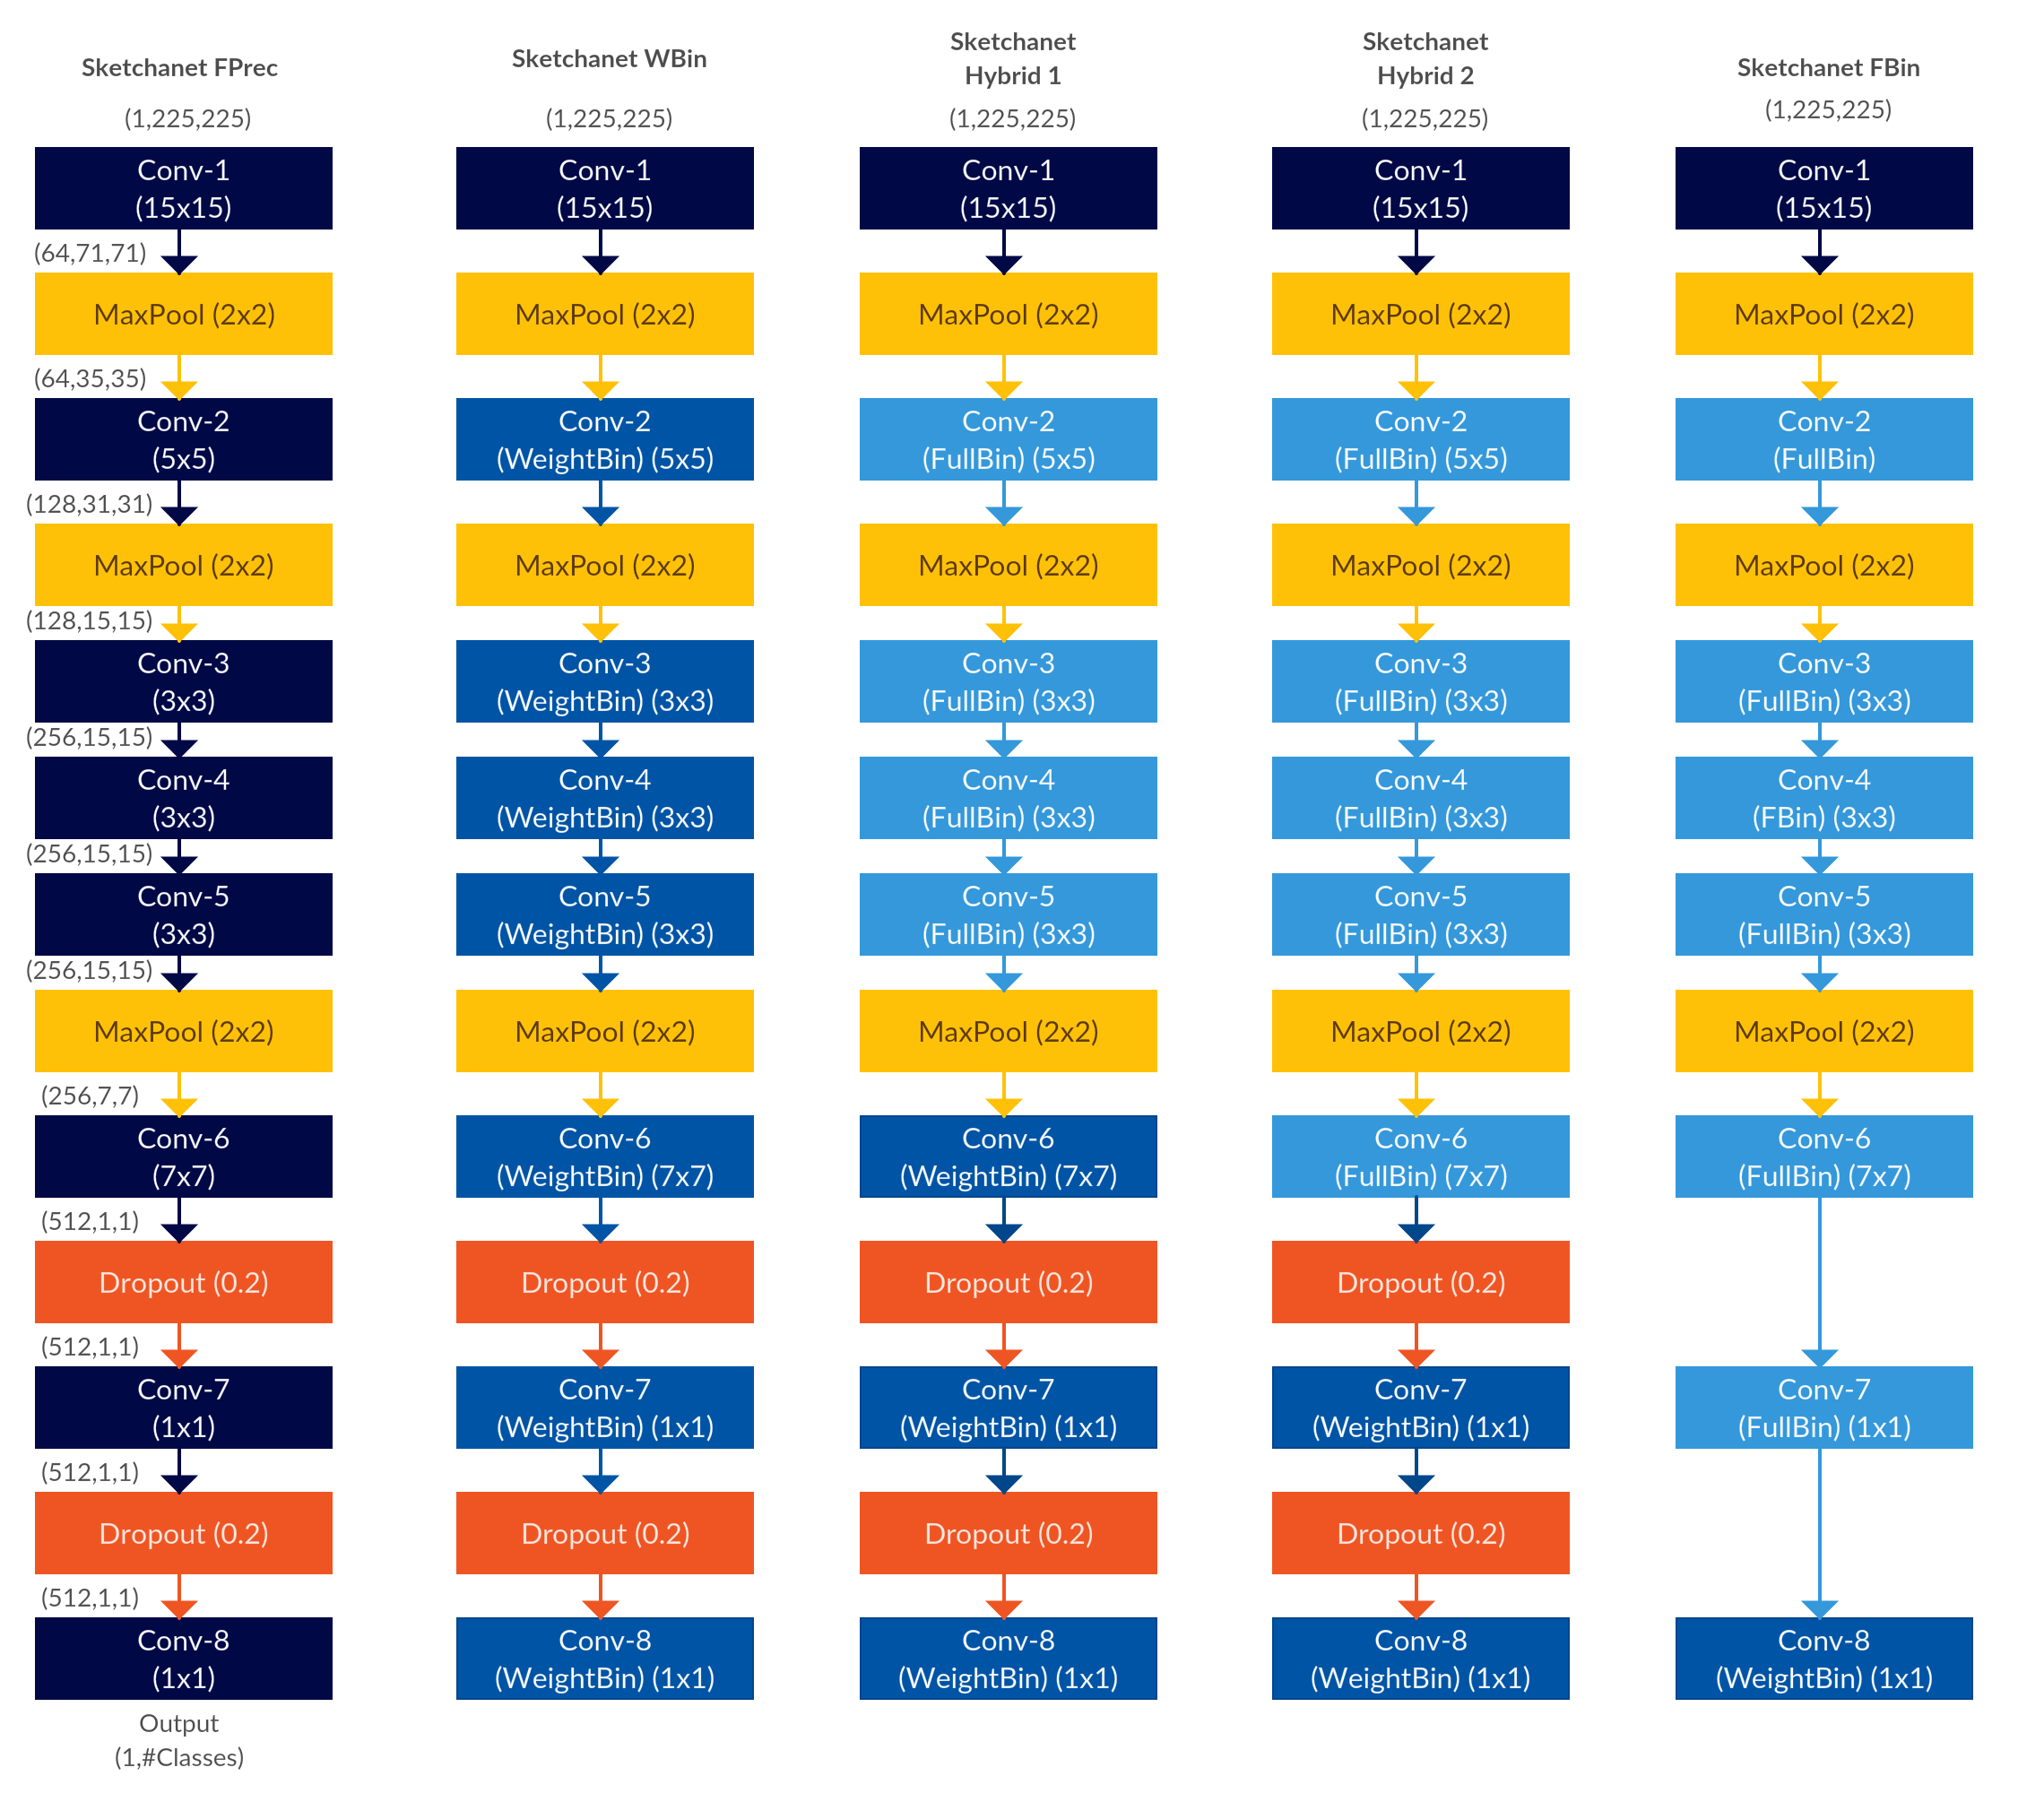
\includegraphics[]{Sketchanet-Final.png}\\
}
\caption{Comparing architectures of FPrec, Wbin, Fbin, and two Hybrid versions of Sketch-A-Net. Our hybrid versions replace most conv layers with FullBinConv layers, but replace layers towards the end with WeightBinConv layers, following the algorithm.}
\vspace*{-0.5cm}
\label{fig:sketchanet}
\end{figure*}

\begin{figure*}[t]
\resizebox{\textwidth}{!}{
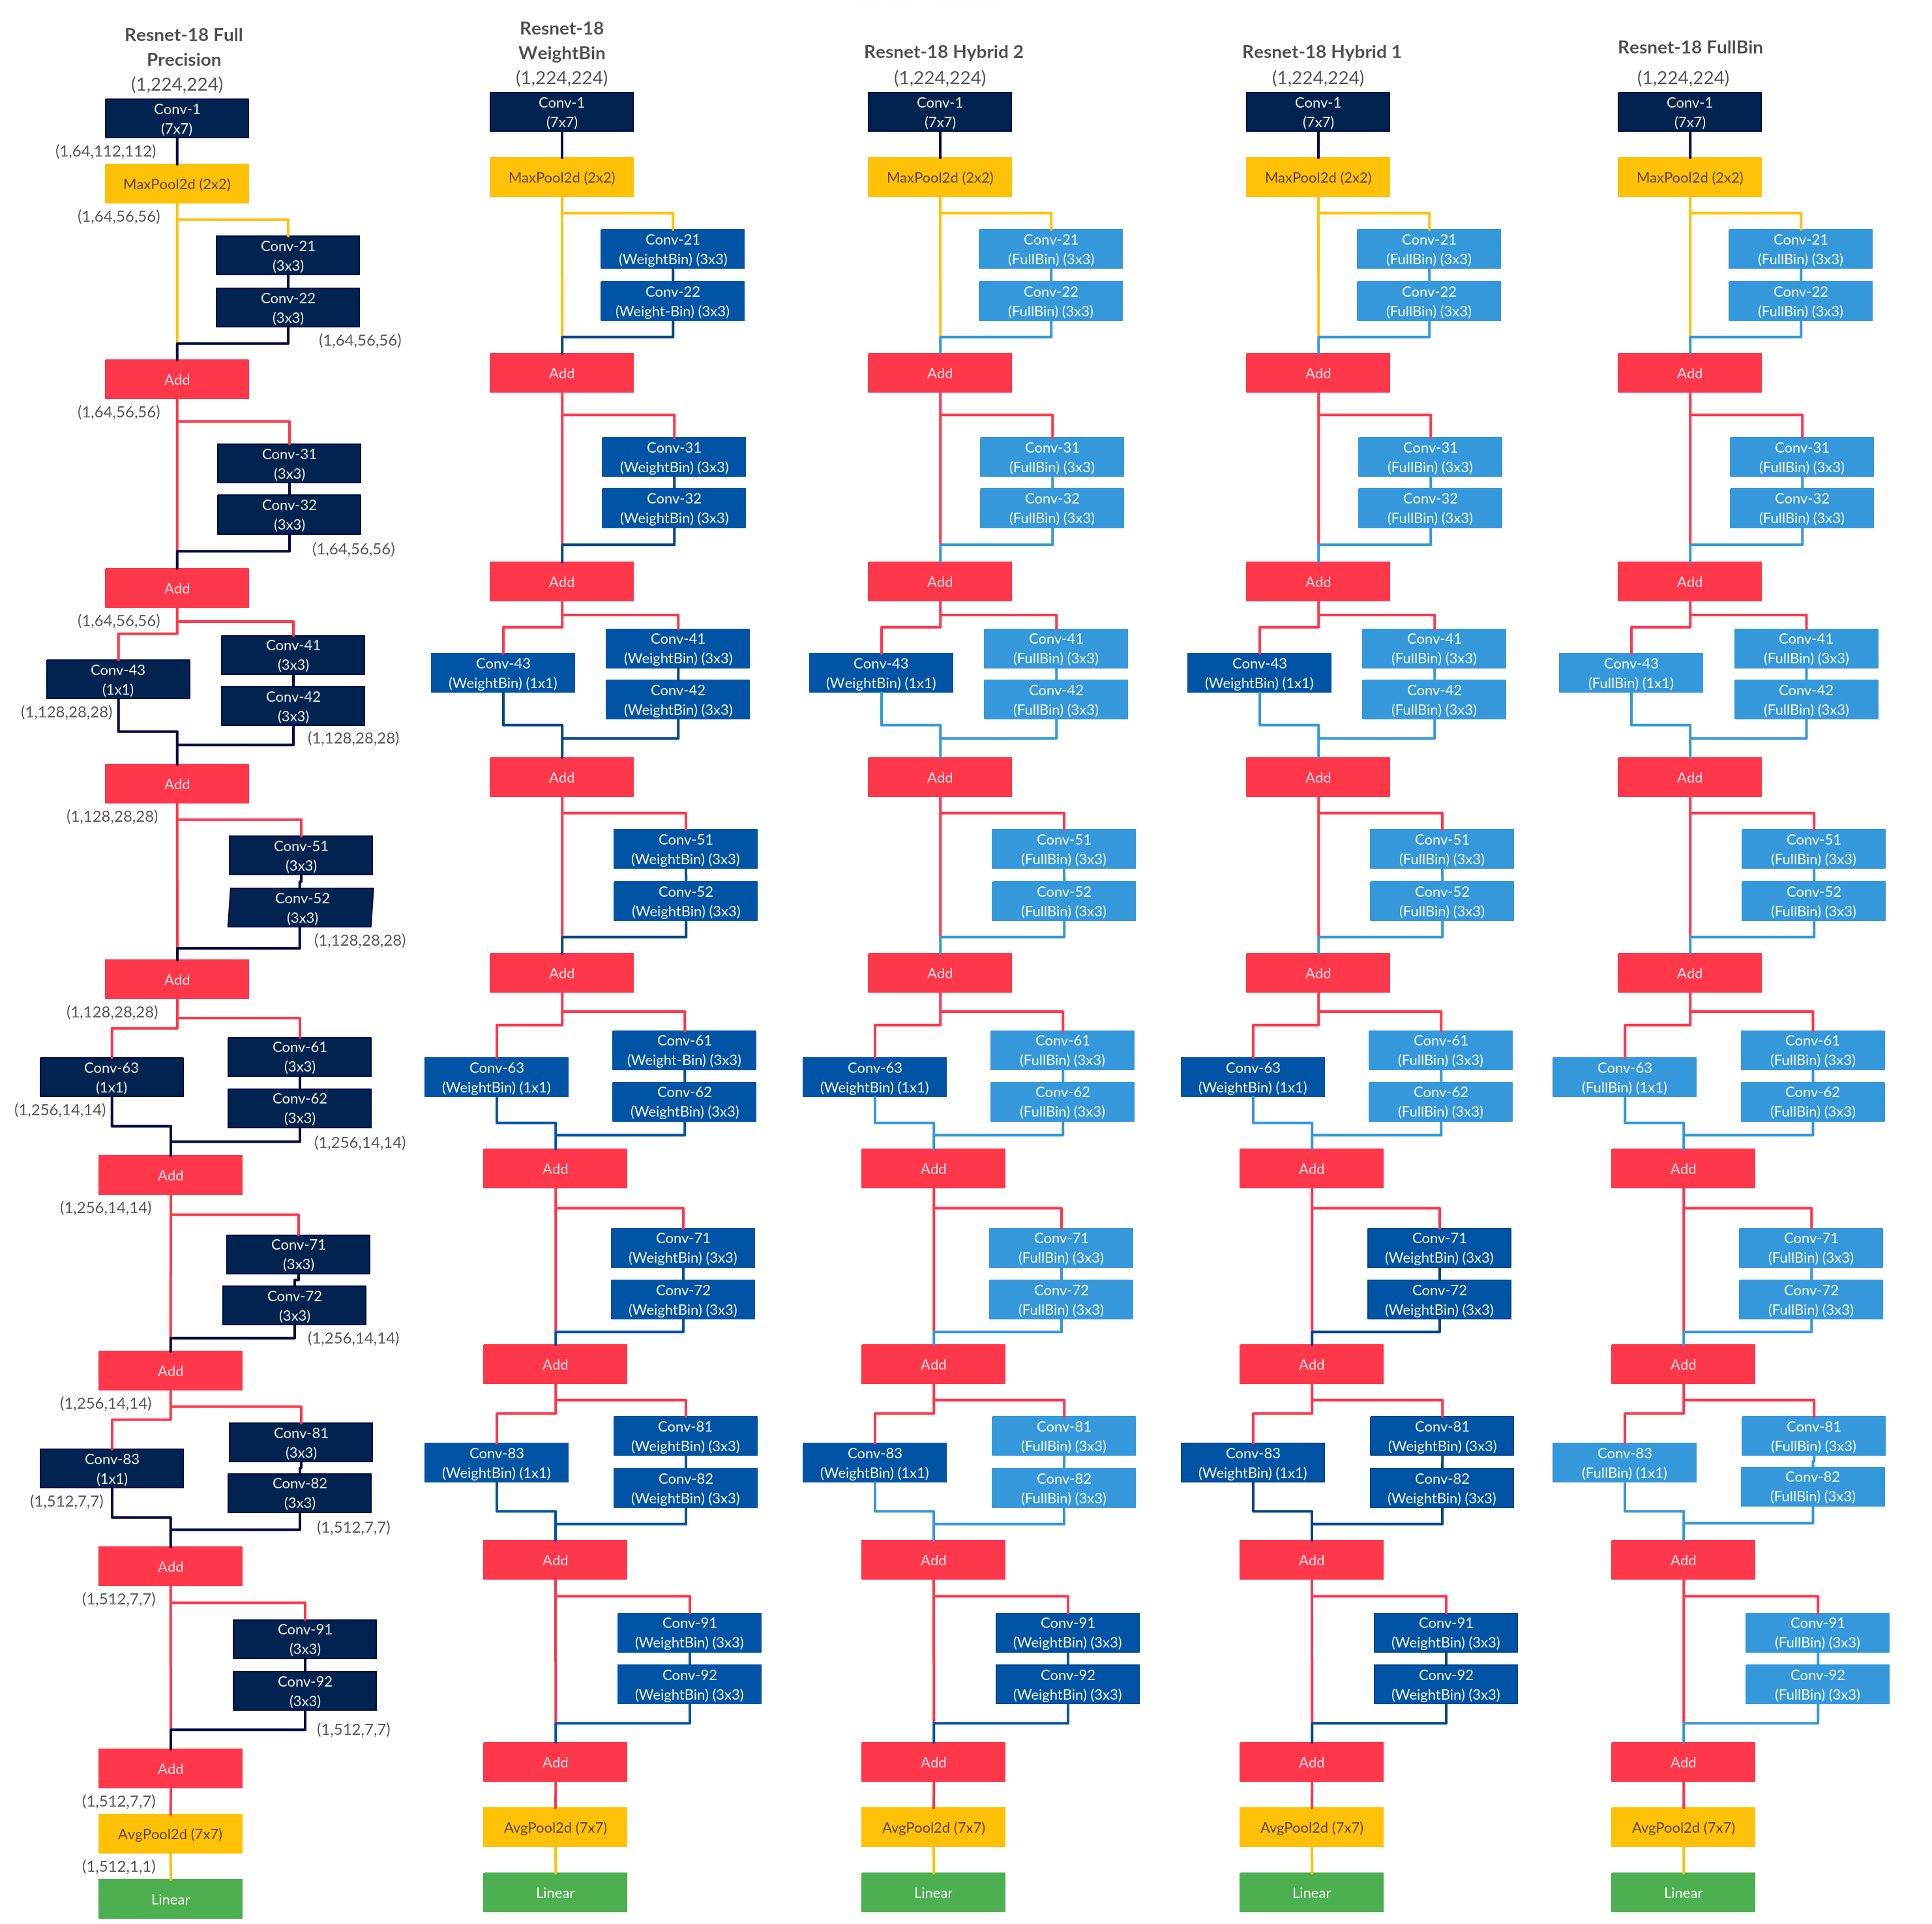
\includegraphics[]{Resnet-Final.png}\\
}
\caption{Comparing architectures of FPrec, Wbin, Fbin, and two Hybrid versions of ResNet-18.}
\label{fig:resnet}
\end{figure*}

\begin{figure*}[t]
\resizebox{\textwidth}{!}{
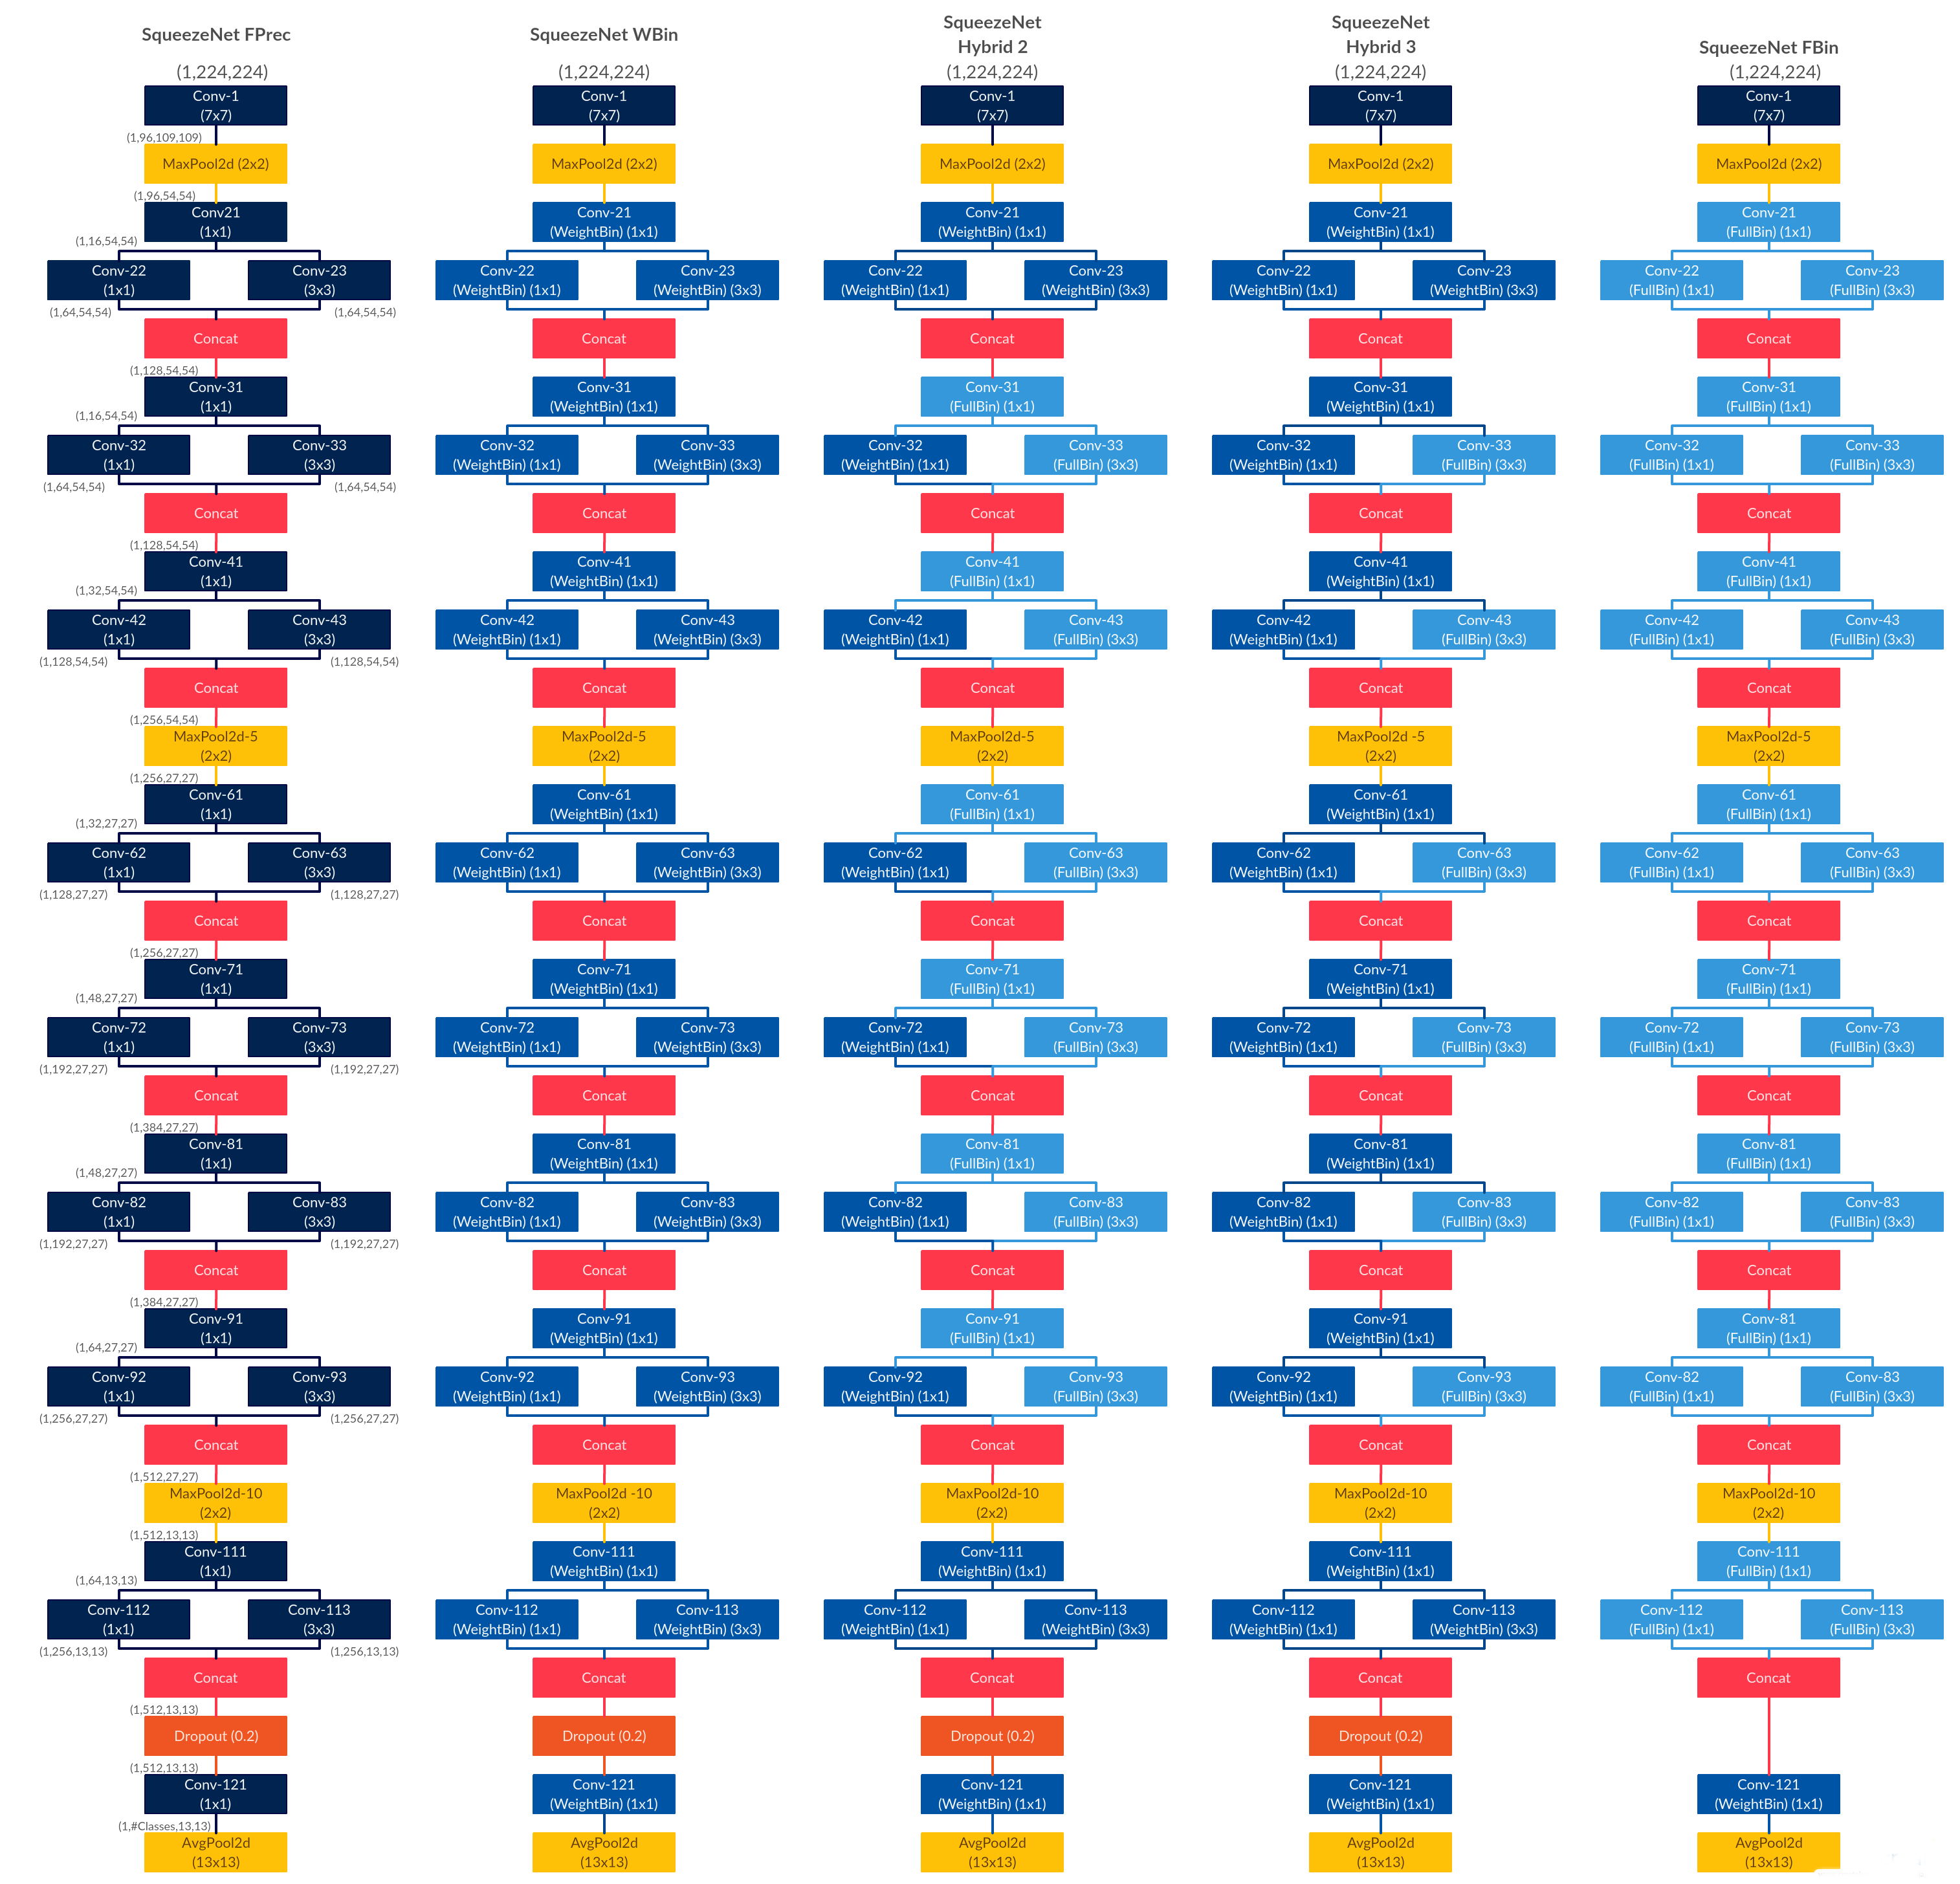
\includegraphics[]{Squeezenet-Final.png}\\
}
\caption{Comparing architectures of FPrec, Wbin, Fbin, and two Hybrid versions of SqueezeNet.}
\label{fig:squeezenet}
\end{figure*}

\begin{figure*}[t]
\resizebox{\textwidth}{!}{
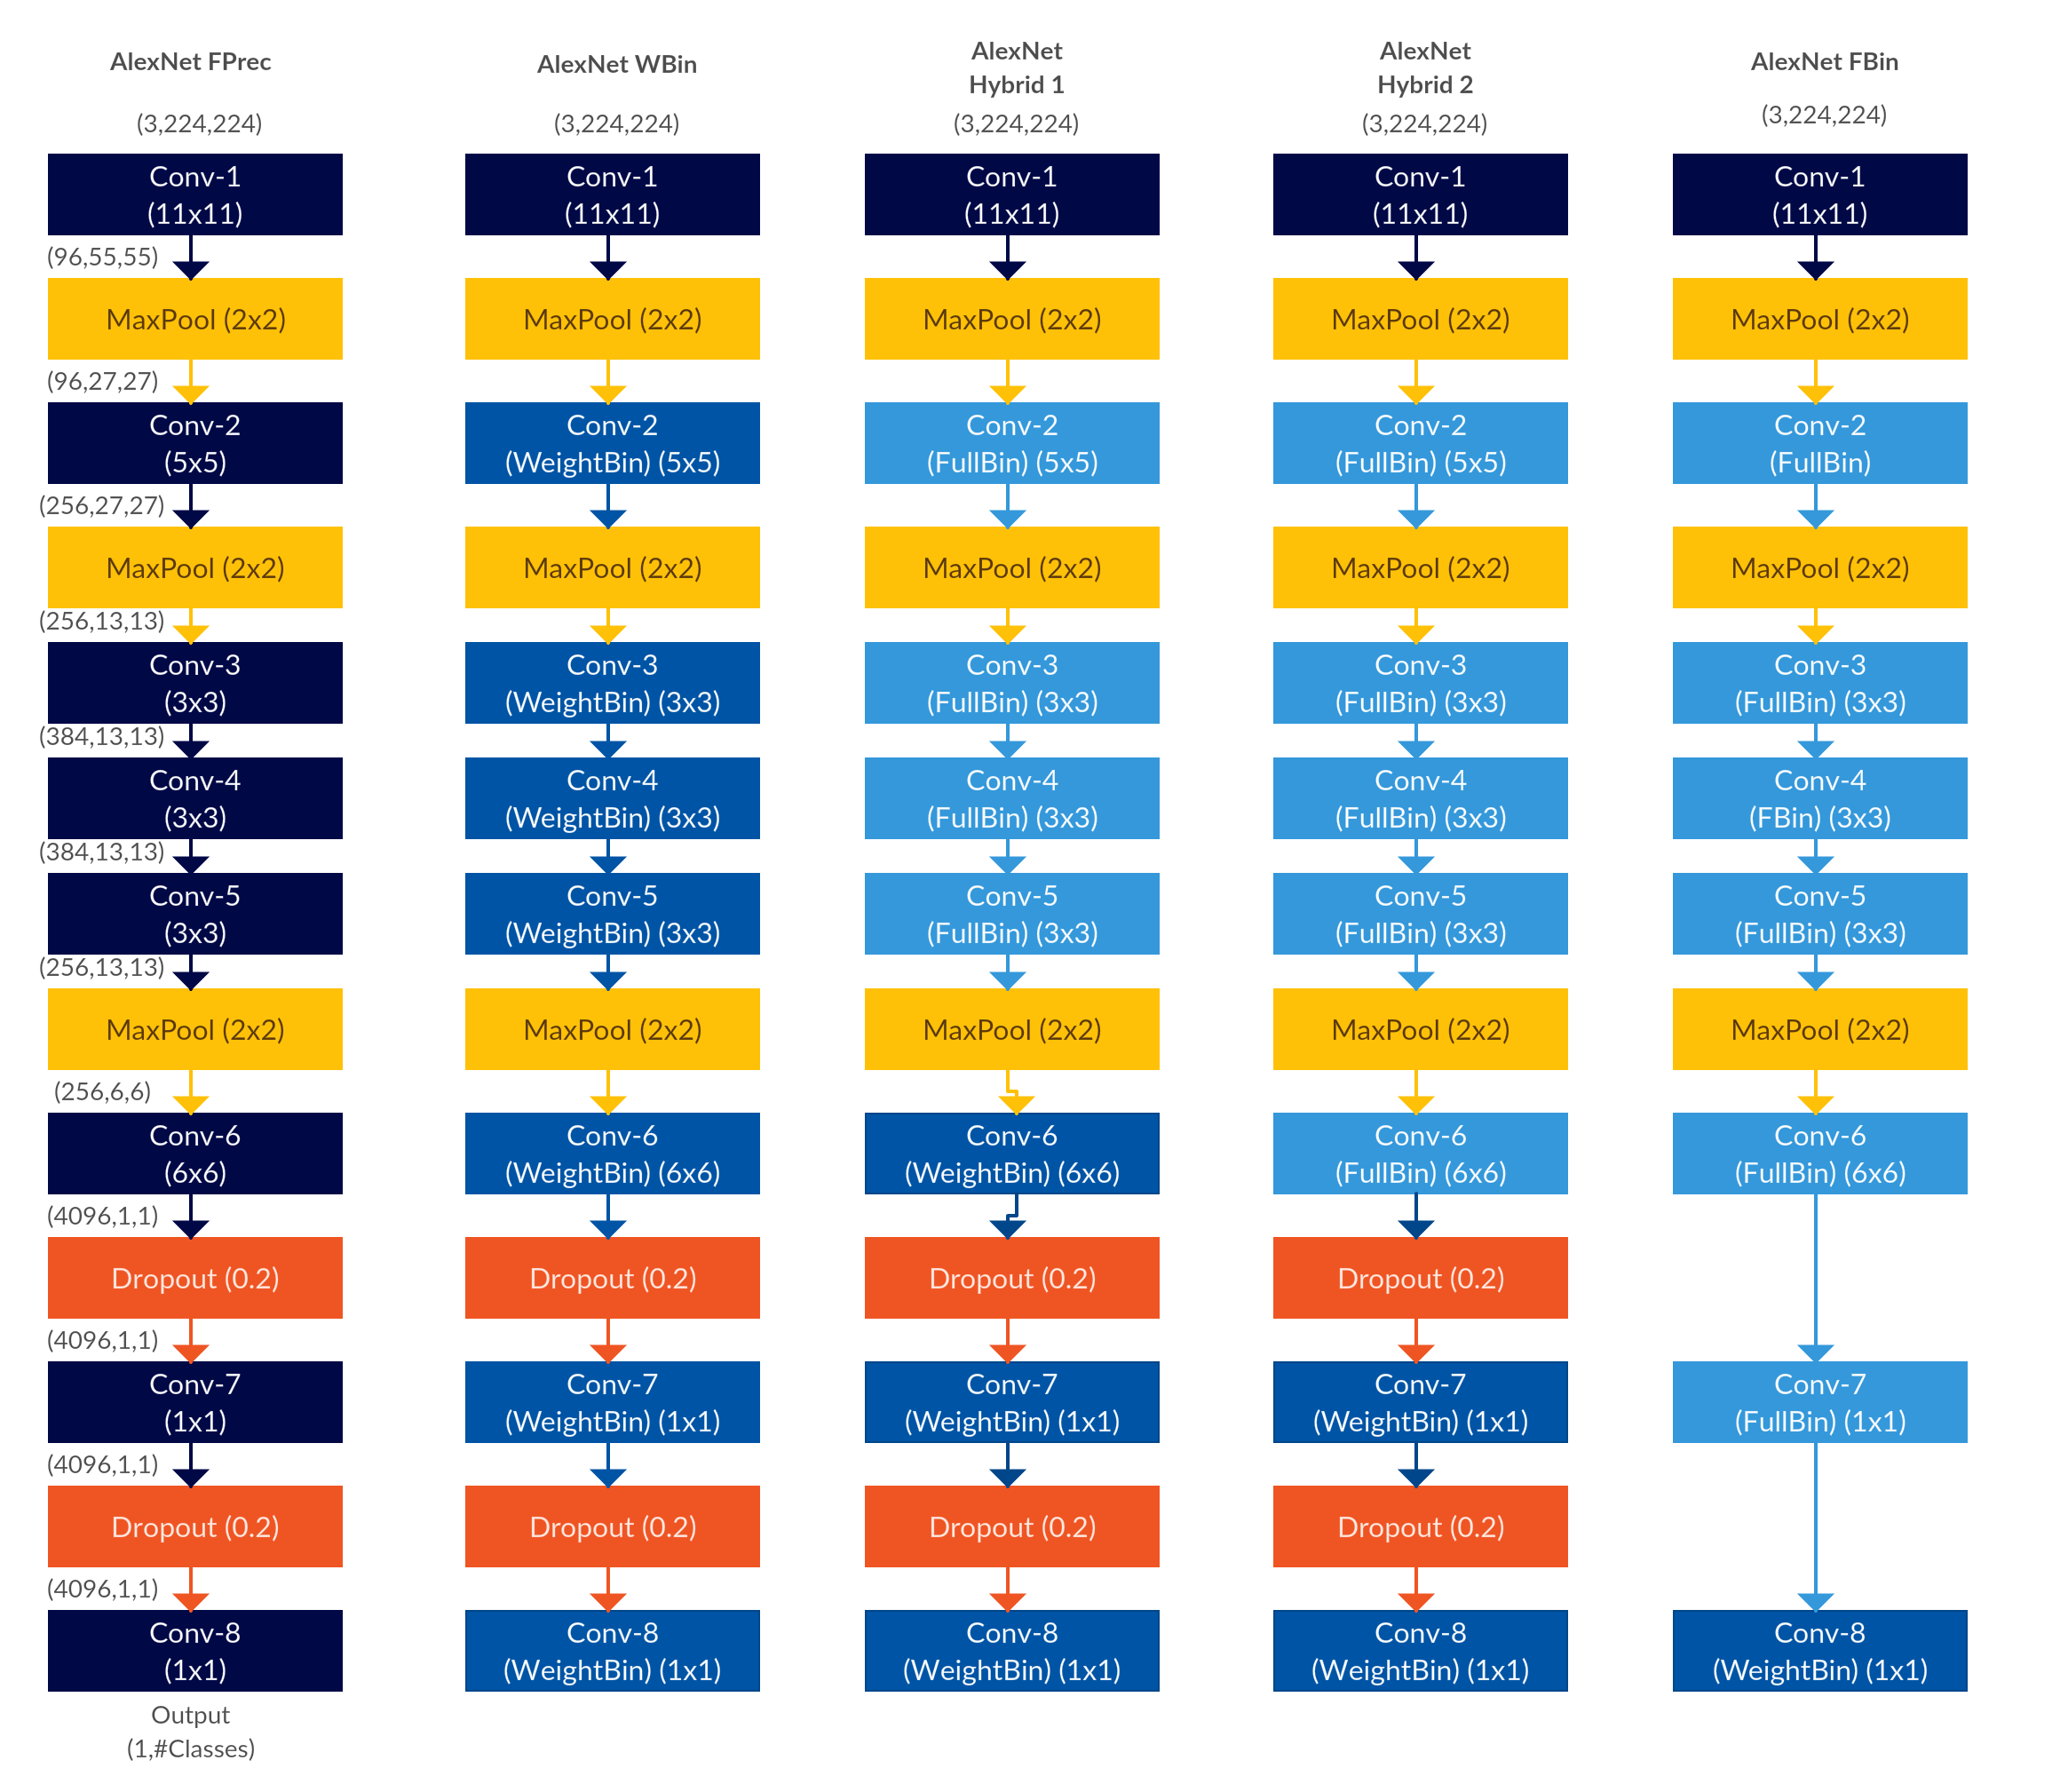
\includegraphics[]{AlexNet-Final.png}\\
}
\caption{Comparing architectures of FPrec, Wbin, Fbin, and two Hybrid versions of AlexNet.}
\label{fig:alexnet}
\end{figure*}